\chapter{Configurable Timed CEGAR} \label{chap:timed_cegar}

This chapter presents a configurable framework for CEGAR-based reachability analysis of timed automata. 

\section{Generic CEGAR Framework}

The key idea of the framework is to provide various implementations of each phases of the CEGAR-loop, by using correspondent parts of CEGAR-based reachability algorithms. Most of these algorithms already exist (mostly for other formalisms, and they have to be adapted to timed automata), but some of them are new approaches. The implemented modules can then be combined (that is, the implementation of each phases can be provided by different algorithms) to form new algorithms, and chosing the most effective parts of the original algorithms can result in an even more effective algorithm then the original ones. \todo{diszkrét változókat megemlíteni}

The architecture of the framework is illustrated on \todo{ábra: (két résszel az automatáshoz és az állapottereshez) amin látszanak hogy pontosan mik lesznek a dobozok (milyen interfészek) és mi megy köztük a nyilakon, stb}. As one can see, there are two different realization of the CEGAR-loop. The reason for this is that not all implementations of the CEGAR-phases can be used interchangably, since there are two distict ways CEGAR-loop can be applied to timed automata. The key difference is the basis of the refinement. While the first approach \todo{ábra a) részét referálni} starts from a pure automaton (without any clock variables) and extends the current automaton with some clocks in each iteration \todo{háttérismereteknél referálni} - and thus refines the \emph{automaton}, the other \todo{ábra b) részét referálni} is based on the refinement of the \emph{statespace} itself. Because of this, only algorithms of the same approach can be combined.

\subsection{Automaton-based refinement}

\todo{Fig ... depicts the architecture...} The initial abstraction is a finite automaton that is derived from the original timed automaton by removing all clock variables and clock constraints. 

In each iteration of the CEGAR-loop, the task of the model checking phase is to determine whether the error location is reachable in the current automaton and provide a trace (counterexample) if there is one. Therefore, the implementation should be a reachability-checking algorithm for timed automata that can find a trace to the location.

The task of the analysis phase is to check if the found trace is feasible in the original automaton and if it isn't, provide a set of clock variables that can then be added to the automaton (with the clock constraints they appear in) so that the model checker won't find this counterExample again. his is quite a complex task and therefore there aren't many implementations of it.

Finally, the only task of the refinement phase is to refine the current abstraction of the automaton, by extending it with the given set of clock variables (and the constraints they appear in). The task is straightforward, and so this part of the CEGAR-loop has only one implementation.

\todo{A pseudocode is provided to demonstrate implementability.}


\subsection{Statespace-based refinement}

In case of statespace-based refinement, the representation of the statespace has a defining role. In the proposed framework, the statespace is represented by zone graphs - this is common for all algorithms. However, the abstraction of the zone graph can be performed various ways. In this framework, the main idea is to explore the statespce without considering clock variables (and in some cases discerete variables, too), and to refine the statespace - trace by trace - by deciding which of the clock variables to include for each of the zones on that path. Afer that the graph is refined (clocks are included in the zones), and during the refinement iut turns out whether the counterExample is feasible or not. \todo{Fig ... depicts the architecture...} 

Because of the different approaches of abstraction, consructing the initial abstraction is not as straightforward as it was in the automaton-refinement phase. All that can be said is that it is some sort of abstraction of the statespace derived from the automaton without including clock variables.

The task of the model checking phase is to find a path from the initial location to the error location in the current abstraction of the zone graph. Because of this, the model checking phase of statespace-based refinement is a pathfinding algorithm.

The task of the analysis phase is to decide which of the clock variables to include in the zones on the trace so that it becomes possible to find out whether or not the counterexample is feasible. The result of the analysis should be a function $P: V(G) \to 2^\mathcal{C}$ assigning a set of clocks to the nodes of the current abstraction of zone graph. This set of clocks can be callled the \emph{precision} of the zone.

The task of the refinement phase is to calculate the zones on the trace (up to the given precision) and find out if it was feasible or not. This can be performed by the steps of the algoorithm presented in \todo{utalás háttérismeretek megfelelő részére} with some modifications that help with handling the changes of precision along the counterexample. If the error location is unreachable, a guard or invariant will eventually prove to one of the edges on the trace that it is not enabled. The current abstraction of the zone graph must be modified accordingly.

\todo{A pseudocode is provided to demonstrate implementability.}

The presented methods for model checking and refinement describe the essence of the algorithms that seem to be the same, however, the concrete implementation depends of the structure of the abstract zone graph representation. Because of this only those modules can be used interchangably, that are defined for the same representation.


\section{Modules}

This section describes the implementations of the previously defined interfaces - grouped by the base of refinement.

\subsection{Implementations for automaton-based refinement}

%\subsubsection{Model checking phase}

First, model checkers are presented that can be used for the model checking phase of CEGAR algorithms with automaton-based refinement. Secondly, an algorithm is defined for calculating the set of clock variables to refine the automaton, and finally, the general algorithm is described for performing the refinement.

\subsubsection{Zone graph exploration} 

The reachability-checking algorithm described in section \ref{sec:tareach} is an obvious choice for the model checking phase, however, it is important to note that the algorithm does not handle discerete variables. The discrete valuation can be encoded into the location (and calculated on the fly) but in this case termination is not ensured (as section \todo{ref} explains).

\subsubsection{Satisfiability-based model checker}

Satisfiability-based model checking was introduced in \todo{background ref}. The idea can be directly applied to timed automata -- the only necessary change is to define transformation that can turn a counterexample (an execution trace) into a SAT-problem.

The idea is to separate discrete transitions from time transitions. Consider a counterexample sequence $\sigma = l_0 \xrightarrow{t_0} l_1 \xrightarrow{t_1} \cdots \xrightarrow{t_n} l_{err}$.  This representation of $\sigma$ hides the fact that it is important how much time the systems spends in each locations - i.e. delay transitions. Let us denote the amount of time spent in $l_i$ by $d_i$. This way $\sigma$ can be defined by $\sigma = l_0 \xrightarrow{d_0} \xrightarrow{t_0} l_1 \xrightarrow{d_1} \xrightarrow{t_1} \cdots \xrightarrow{d_n} \xrightarrow{t_n} l_{err}$. In this representation $\xrightarrow{d_i}$ can be considered a special kind of transition that increases $v(c)$ for each $c \in \mathcal{C}$ by $d_i$. Based on this the SAT formula can be constructed.

First, let us assign a variable for each clock in each location, both before and after the delay -- that is, this means $2\cdot n \cdot \abs{\mathcal{C}}$ variables. Let us denote these variables by $c_i$ (for the value of clock $c$ in location $l_i$ before the delay) and $c_i'$ (for the value of clock $c$ in location $l_i$ after the delay). Let us also assign variables for each $d_i$. The first constraints that have to be added is that each of the defined variables are greater or equal to 0.

The initial constraints can simply be described by $c_0 =0$ for each $c \in \mathcal{C}$. Delay transitions can be turned into constraints by the following equation $c_i+d_i=c_i'$ for each $c \in \mathcal{C}, 0 \leq i \leq n$. In case of discrete transitions, guards (clock constraints) can be turned into \todo{solver constraints?} by replacing the clock variables with the defined variables. The guard $g_i$ of a transition $t_i(l_i,g_i,r_i,l_{i+1})$ can be transformed by replacing all clocks $c$ appearing in $g_i$ by $c_i'$. Resets can also be simply transformed into constraints -- for all $c \in r_i$ $c_{i+1}=0$ has to be added to the set of constraints. Note, that this way $c_{i+1}$ is only specified for the reset clocks. For all $c \not \in \r_i$ $c_{i+1}=c_i'$ has to be added to the set of constraints. Invariants can be transformed into \todo{solver constraints?} the same way as guards.

Discrete variables can be mapped to \todo{solver variables?} as before since discerete variables and clock variables have no effect on eachother.

\todo{példa}

This allows us to use a SAT-solver to decide if a possible execution trace of a timed automaton is feasible. This can be used for model checking timed automata, by iterating over all possible execution traces and if a trace $\sigma$ is found from $l_0$ to $l_{err}$, it can be checked, and if the derived formula is satisfiable, $\sigma$ is proposed as a counterexample. 

The problem with this model checker is that there may be infinitely many execution traces. Thus, this model checker can only be used as a \emph{bounded} model checker \todo{háttérismerekhez ez is}.

\todo{A pseudocode is provided to demonstrate implementability.}

\subsubsection{Unsat core-based clock selection}

Solvers can be useful, not only to decide if a given set of constraints is satisfiable, but also - if the answer is \emph{unsat} - solvers have various features to show why they can not be satisfied. One of the possible helpful feature is deriving the so called \emph{unsat core} - that is, a minimal set of the given constraints that is unsatisfiable in itself. This set of constraints can be used to determine the set of clock variables with what the current abstraction of the automaton has to be extended. In order to define the refinement set, the variables appearing in the unsat core have to be transformed back to the original variables. The set of original variables appearing in the constraints is the result of the algorithm.

\todo{példa}

\todo{pszeudokód?}

\subsubsection{Automaton refinement}



\todo{a végére ábra az elkészült dobozokról.}

\subsection{Implementations for statespace-based refinement}

\subsubsection{Abstractions} % ezt lehet jobb lenne nem subsubsecionként?

\subsubsection{Statespace exploration}

\subsubsection{Trace Activity}

\subsubsection{Unsat core-based precision}

\subsubsection{Statespace refinement}

%Implementált modulok felsorolva, utalással az előző fejezet algoritmusaira. + példák, pszeudokód


\section{Combined Algorithms}
A fenti modulok kombinálhatósága. Ekészült algoritmusok.

%\subsection{Timed automaton-based refinement with sat based mocdel checker}
%\subsection{Timed automaton-based refinement with sat based mocdel checker}

%
%\todo{Algoritmusok, leírással, hol használják, hogyan lehet TA-ra alkalmazni, miért jó, stb. + hogyan fog beleilleszkedni a konfigurálható izébe (milyen dobozok)}








%\todo{Elkészült dobozok, intefészek, kombinálhatóság}

%\section{}

%\section{Introducing a new algorithm}

%\todo{El kéne nevezni ezt az algoritmust és akkor nem kellene mindenhol "az X. fejezetben bemutatt algoritmus"-ként hivatkozni rá.}

%My algorithm is explained in this section. To ease understanding it is also demonstrated on the automaton in Figure \ref{fig:loopinfinite}, with the error location being the location $end$.

%\subsection{Overview}

 %Due to these disadvantages discussed above I have decided that my approach of applying CEGAR to the reachability analysis of timed automata will modify the reachability algorithm instead of using it as a black box module. My approach applies abstraction to the zone graph of the automaton, instead of the automaton itself. The reachability algorithm (which will now be a CEGAR-based algorithm) will refine the zone graph iteration by iteration until reachability can be decided. The CEGAR loop is interpreted the following way.

 %\begin{description}
 %	\item[Initial abstraction] The key problem about constructing the initial abstraction of the zone graph is that the zone graph is unknown so the abstraction has to be derived from the automaton itself. The idea is really simple: just like the other approaches I also use the location graph of the automaton as the initial abstraction, except in my algorithm it is considered to be the abstraction of the zone graph, not the automaton. To create an overapproximation of the zones, we simply consider every valuations to be reachable in all locations. The zone containing all valuation is denoted by $z_\infty$.
 %	\item[Model checking] Since the abstract zone graph is an abstraction of the reachability graph, model checking becomes a pathfinding problem in the current abstraction of the zone graph. The error location is either proven unreachable or a new trace (path in the graph) is found from the initial node to the target node.
 %	\item[Analysis] This part is about finding out if the error location is really reachable on the trace found in the model-checking phase. The way to do that is by finding out how this path of the abstract zone graph would look like in the refined (real) zone graph. This can be achieved by using the reachability algorithm, but only for the given trace. As discussed in Section \ref{sec:reach}, because of the operation \emph{split} sometimes the real zone graph can branch, which means that the result of the simulation may be a tree instead of a simple path. Nevertheless, it is still easy to decide whether the counterexample is valid: if the error location could be reached by the path (on any branch), then the counterexample is valid. Otherwise, simulation will stop somewhere, typically because one of the transitions (on each branch) is not enabled. In this case the counterexample is spurious.
 %	\item[Refinement] In order to avoid the discussed disadvantages, this algorithm stores as many information of the analysis phase as it can - by replacing the counterexample trace in the abstraction of the zone graph with the calculated subgraph (tree) -- thus refining the abstraction.
 %\end{description}

 
 %\begin{figure} [h]
 %	\centering
 %	\begin{minipage} {0.2\linewidth}%
% 		\vspace*{10pt}%
% 		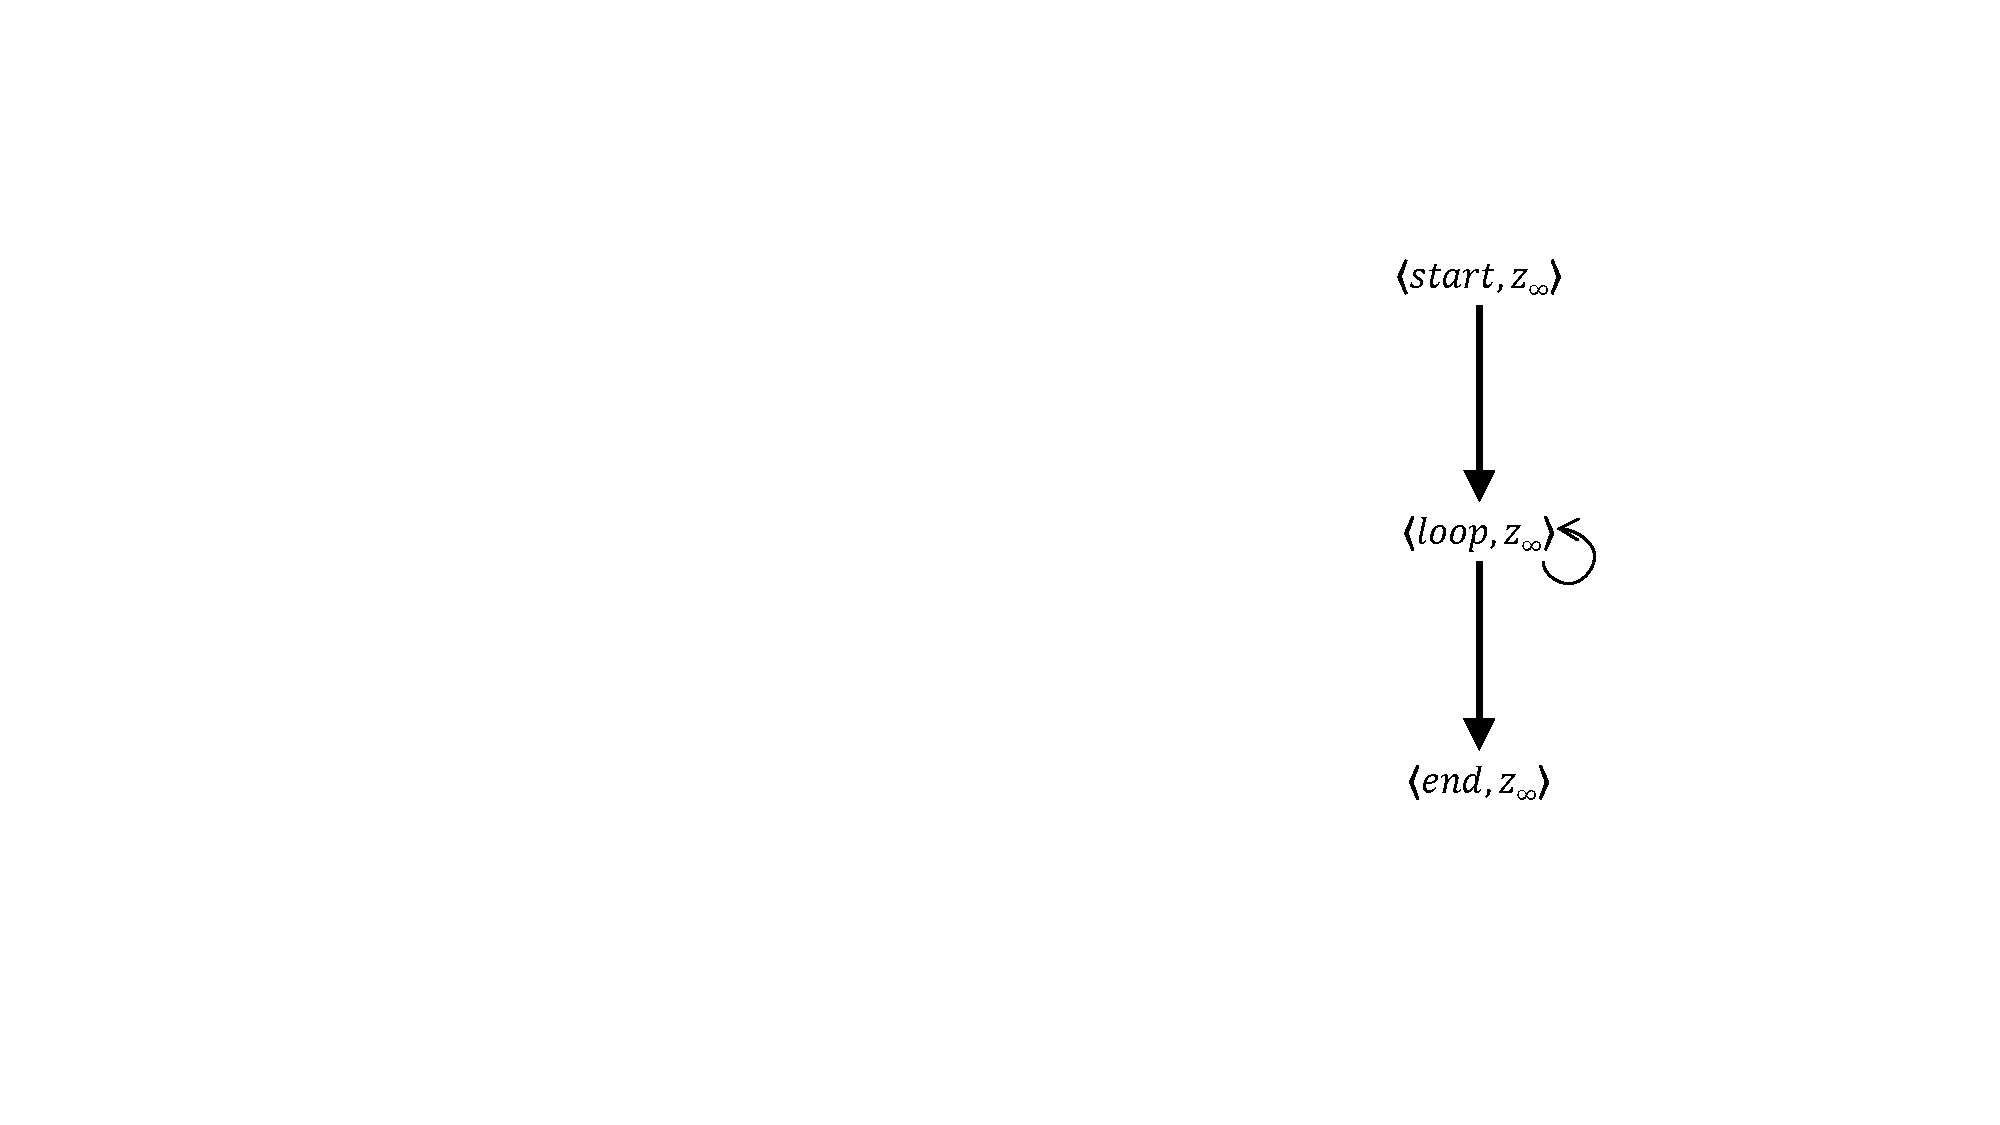
\includegraphics [width=\textwidth]{include/figures/loop_initial_abst}%
% 		\caption{Initial abstraction}
% 		\label{fig:x}
% 	\end{minipage}%
% 	\hspace{20pt}	%
% 	\begin{minipage} {0.2\linewidth}%
% 		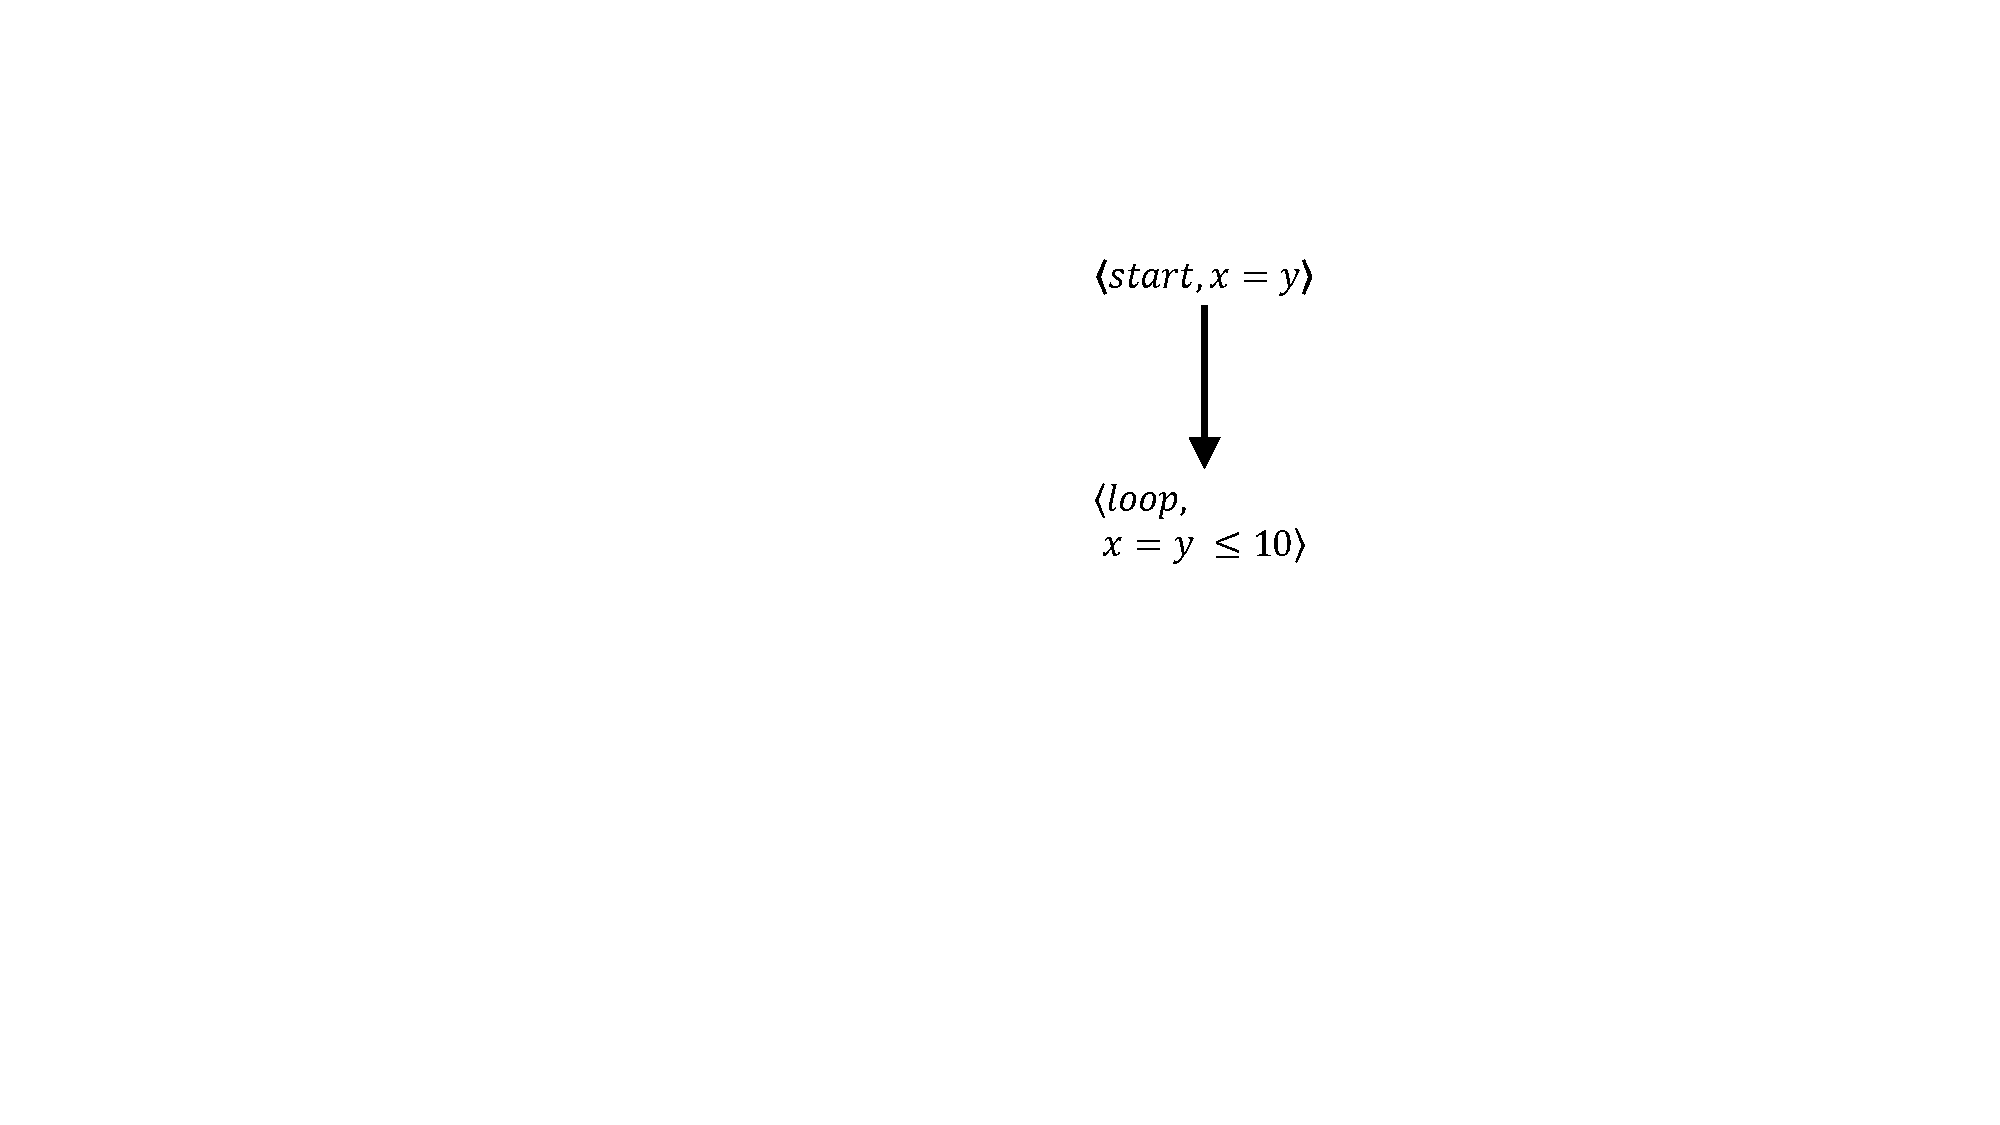
\includegraphics [width=\textwidth] {include/figures/loop_first_ref}%
% 		\vspace*{103pt}%
% 		\caption{Result of analysis}
% 		\label{fig:loopanal}
% 	\end{minipage}%
% 	\hspace{20pt}%
% 	\begin{minipage} {0.25\linewidth}%
% 		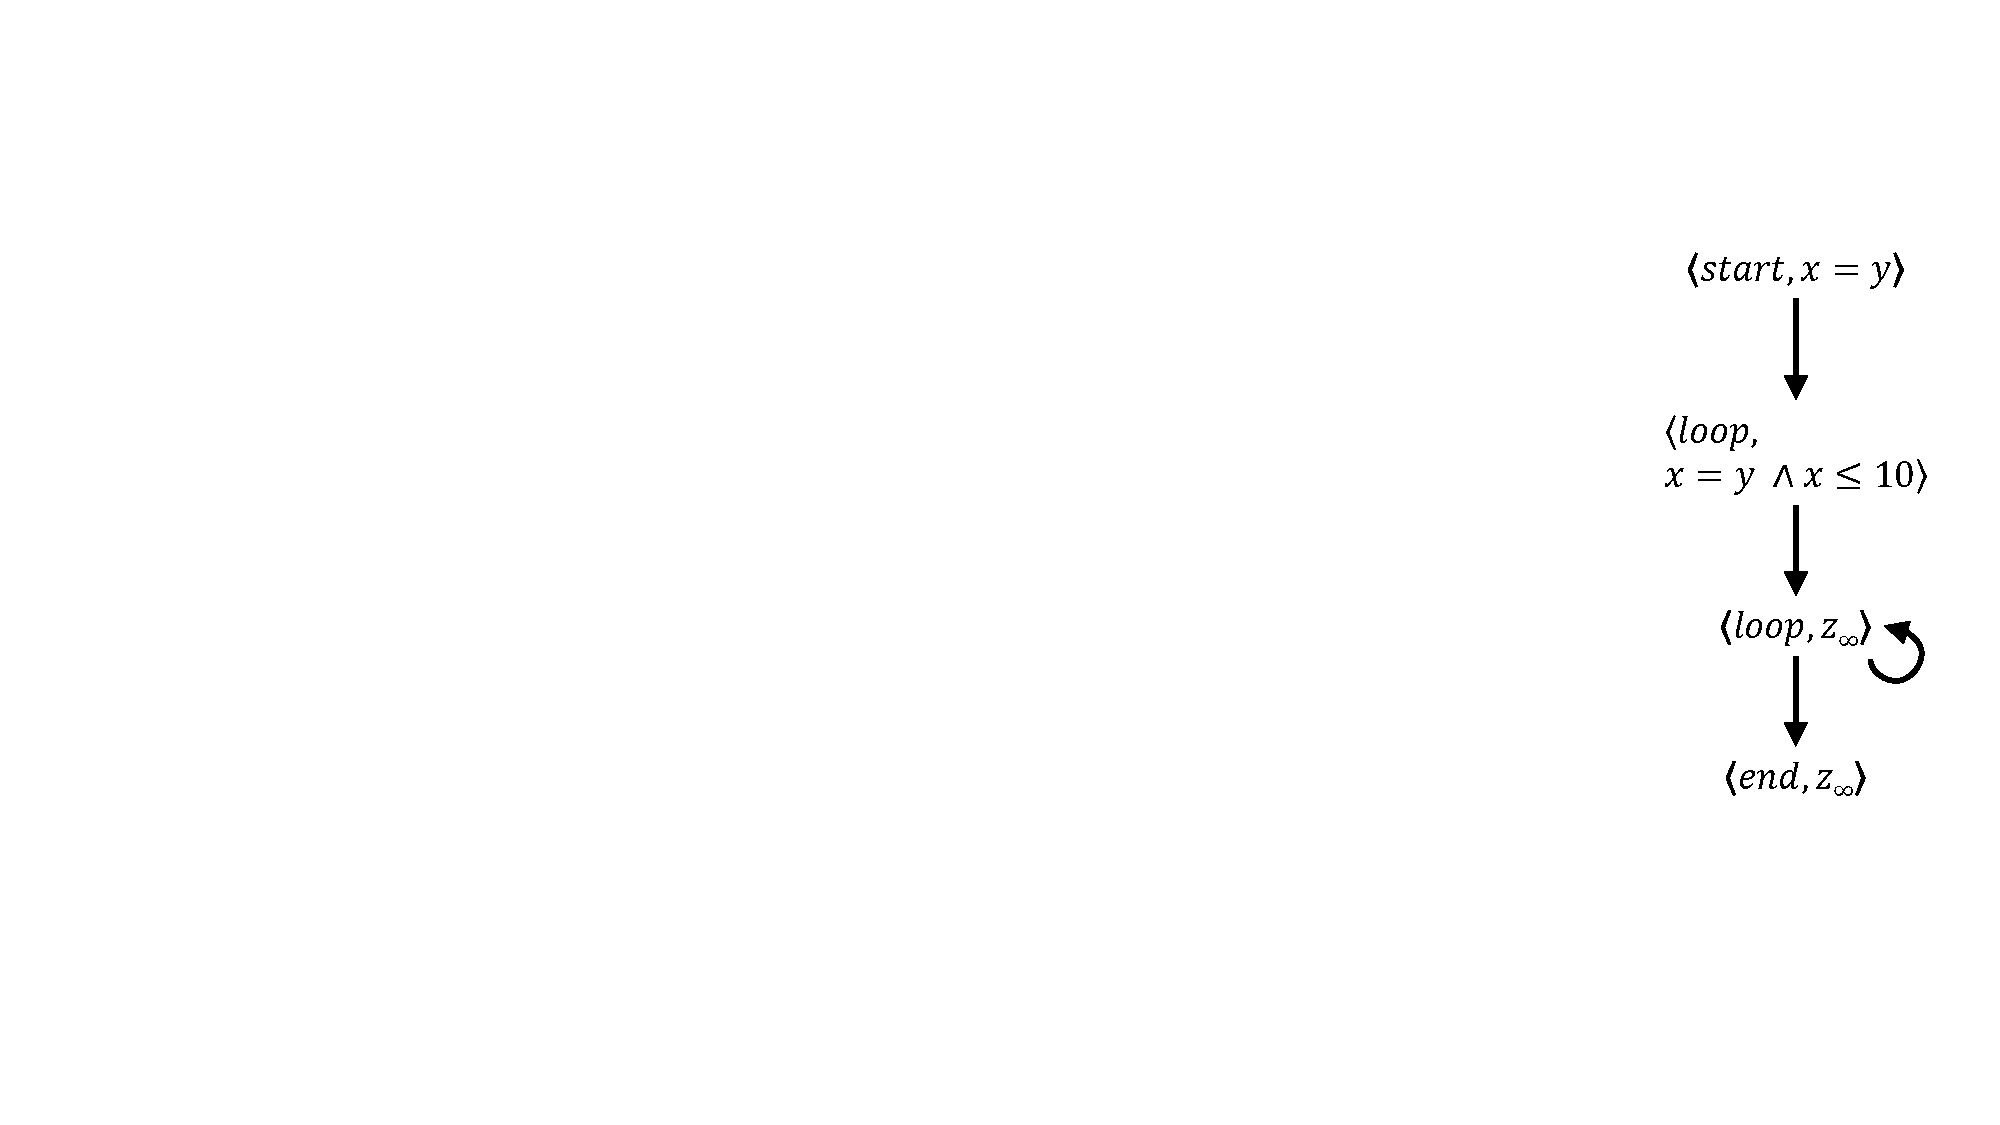
\includegraphics [width=\textwidth] {include/figures/loop_first_abst}%
% 		\vspace*{5pt}%
% 		\caption{After refinement}
% 		\label{fig:loopref}
% 	\end{minipage}
% 	\caption{Timed CEGAR on an example}
% \end{figure}
% 
 
%\subsection{Details}
%
%It is very important to perform the presented operations correctly. This section explains the algorithm step by step, demonstrating it on the example automaton in Figure \ref{fig:loopinfinite}.
%
%Constructing the initial abstraction is very straightforward: each node of the location graph are to be completed with the zone $z_\infty$. After that, model checking is simply a pathfinding in the current abstraction of the zone graph.
%
%\begin{example}
%	The initial abstraction of the example automaton's zone graph is depicted in Figure \ref{fig:x}. The first counterexample is denoted with bold arrows.
%\end{example}
%
%Simulation of the counterexample is performed by constructing the relevant part of the real zone graph. In the first iteration each node on the path will contain $z_\infty$. In this case, refinement starts from the node that belongs to the initial location and the refined zone is calculated as the initial zone of the zone graph.
%
%The result of pathfinding in the graph in Figure \ref{fig:x} is denoted by bold arrows. In case of the later iterations the first few nodes of the
%trace will already be refined, so the refinement can start from the first
%abstract node. The reachable zone should be calculated from the last refined zone,
%considering the guards and the reset as when constructing the zone graph.
%
%When the result of the refinement is more than one zone, the node on the path (and the edge pointing
%to it) is replicated, and one of the refined zones are assigned
%to each resulting node. The refinement can be continued from any of these nodes -- the path branches.
%All of these branches should be analyzed (refined) one by one.
%
%If the erroneous location is reachable through this path, the procedure finds it,
%and the CEGAR algorithm terminates. Otherwise, at some point a guard or a target invariant
%is not satisfied -- the transition is not enabled. The corresponding edge is removed and the analysis of the path terminates.
%
%\begin{example}
%	Consider the example. Since it is the first iteration, we start by constructing the initial node, $\langle start, x=y \rangle$. After that we calculate the next node on the trace $\langle loop, x=y \leq 10 \rangle$. When constructing the zone graph, we continued with the transition represented by the loop-edge but this time we only have to explore the zone graph through the transitions in the counterexample. The next transition is the transition represented by the edge directed to node $\langle end, z_\infty \rangle$. This transition is not enabled in the previously calculated zone, which means the counterexample is spurious. The resulting subgraph of the zone graph is depicted in Figure \ref{fig:loopanal}.
%\end{example}
%
%The goal of refinement is to eliminate the spurious counterexample from the abstract representation. Refinement is applied by replacing the abstract counterexample with the subgraph of the real zone graph calculated in the \emph{Analysis} phase. This operation has to be performed very carefully.
%
%Consider e.g. that the node in the abstract graph that is about to get replaced by one (or more) nodes in the subgraph has other incoming edges than the one in the counterexample. Since it is unknown what states are reachable in the location by the other incoming edges, the node can't be removed. Except, the edge representing the transition in the counterexample has to be redirected to the node with the calculated zone (if there are multiple nodes, it has to be replicated).
%
%Let us suppose that the graph is prepared to place the new node(s). To avoid wasting memory it is advised to use already refined zones in the graph. If the refined zone $z$ of the node $\langle l,z \rangle$ is a subzone of a zone $z'$ in a node $\langle l,z' \rangle$ (both nodes
%contain the same location $l$), then any state that is reachable from $\langle l,z \rangle$ is also reachable from $\langle l,z' \rangle$, thus there is no need to add  $\langle l,z \rangle$ to the graph. Instead, any edge leading to  $\langle l,z \rangle$ should be redirected to $\langle l,z' \rangle$. After that the replacement of the path can not continue from that $\langle l,z' \rangle$, since there might be more states reachable from $\langle l,z' \rangle$ than from $\langle l,z \rangle$. The remaining of the refined zones have to be recalculated and then the replacement can continue.
%
%When replacing the node, the outgoing edges should also be considered. The calculated subtree of the real zone graph only contained the edges in the trace, but in the abstract zone graph there are other outgoing edges of the node. These edges are the outgoing edges of the original (abstract) node in the zone graph, and they have to be replicated, as outgoing edges from the added node(s). After this we can continue with the next node.
%
%\begin{example}
%In the example replacing the initial node can simply be performed by replacing the zone $z_\infty$ with the zone $x=y$. On the other hand, replacing the node $loop$ has to be performed carefully. Since the loop-edge is an incoming edge of the node and is not part of the counterexample, the node can not be replaced. Instead, the incoming edge on the trace is redirected to the new node (in other words, the one to the original node is removed). Since a new node is added, we have to think about it's outgoing edges that are not on the trace -- in this case the only one is the loop edge. For reasons explained before, the loop edge has to be redirected to the abstract version of the node. Thus, the refinement is finished, and now the counterexample is eliminated from the abstract zone graph. Th resulting graph is depicted in Figure \ref{fig:loopref}.
%\end{example}
%
%
%%\section{Realization}
%
%%\todo{Megvalósítós részek ide + pszeudokód}
%
%\section{Evaluation}
%
%It is important to prove that the algorithm is correct, and that it terminates. Both proof relies on that of the original algorithm.
%
%The algorithm always terminates, because the abstraction of zone graph gets refined in every iteration. Even at worst case, the algorithm stops when the zone graph is completely refined.
%
%The algorithm is correct, because the original algorithm is correct. If the algorithm finds a counterexample, it is a trace in the original algorithm. Otherwise, if there is a counterexample in the original algorithm, this algorithm finds it at some point.
%
%
%
%%\todo{Terminálódás, komplexitás, stb.}
